\documentclass[english]{scrartcl}

\usepackage{babel}
\usepackage{fontspec}
\usepackage{microtype}

\usepackage{csquotes}

\usepackage{amssymb,amsmath,amsthm}

\theoremstyle{plain}
\newtheorem{lemma}{Lemma}

\theoremstyle{definition}
\newtheorem{definition}[lemma]{Definition}

\usepackage[
            backend=biber,
            style=alphabetic,
            isbn=false
        ]{biblatex}

\addbibresource{sources.bib}

% Colors
\usepackage{xcolor}
\definecolor[named]{uboBlue}{cmyk}{1,.7,0,0}
\definecolor[named]{uboYellow}{cmyk}{0,.3,1,0}
\definecolor[named]{uboGrey}{cmyk}{0,0,.15,.55}

\usepackage{tikz}
\usetikzlibrary{calc,positioning}

\newcommand*{\todo}[1]{\textcolor{red}{TODO:~#1}}

\usepackage{suffix}
\newcommand{\citeauthoryear}[1]{\citeauthor{#1} \citeyear{#1}}
\WithSuffix\newcommand\citeauthoryear*[1]{\citeauthor*{#1} \citeyear{#1}}

\newcommand*{\IN}{\mathbb{N}}
\newcommand*{\IZ}{\mathbb{Z}}

\usepackage{mathtools}
\DeclareMathOperator{\smod}{mod}
\DeclareMathOperator{\id}{id}
\DeclareMathOperator{\crt}{CRT}
\DeclareMathOperator{\diag}{diag}

\newcommand*{\crtp}[2][i]{\crt_{(p_{#1})}\left(#2\right)}

\newcommand*{\rand}{\mathcal{R}}

\newcommand*{\pubkey}{\mathrm{pubKey}}

\usepackage{hyperref}
\usepackage{cleveref}

\title{An intro to multilinear maps and their attacks using the example of CLT13}
\author{Lukas Kempf}

\begin{document}
    \maketitle

    \tableofcontents

    \section{Theory of multilinear maps}\label{sec:intro}

    The Diffie-Hellman key exchange is commonly used to derive a secret key between two parties using a public channel. Such an exchange between the two parties Alice and Bob is sketched in figure~1. Alice and Bob decide on a group $G$ with generator $g$. Both choose a secret random integer which they keep secret. Alice calls here integer $a$ and send $g^a$ to Bob; Bob calls his integer $b$ and sends $g^b$ to Alice.
    Now both can derive a shared secret $K = {g^a}^b = {g^b}^a$. This scheme is secure assuming it is hard for an attacker to compute $g^{ab}$ given $g$, $g^a$ and $g^b$. This is known as the Computational Diffie-Hellman assumption.

    \begin{figure}
        \centering
        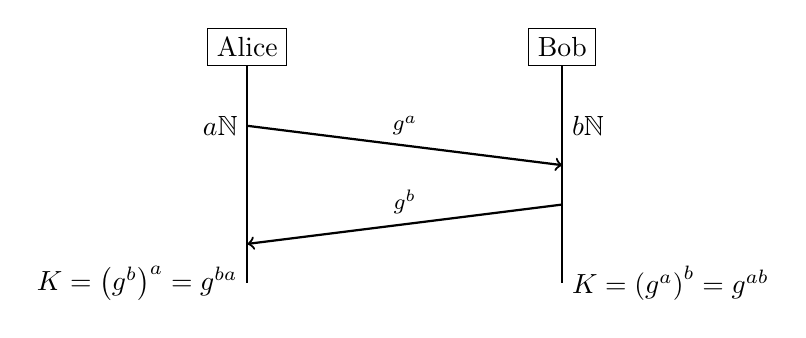
\begin{tikzpicture}
            % Alice
            \node[draw] (Alice) at (-2,0) {Alice};
            \draw[thick] (Alice) -- ++(0, -3);

            % Calculations of Alice
            \node[draw=none,fill=none,anchor=east] (asecret) at ($(Alice) + (0,-1)$) {$a \rgets \IN$};
            \node[draw=none,fill=none,anchor=east] (akey) at ($(Alice) + (0,-3)$) {$K = \left(g^b\right)^{a} = g^{ba}$};

            % Bob
            \node[draw] (Bob) at (2,0) {Bob};
            \draw[thick] (Bob) -- ++(0, -3);

            % Calculations of Bob
            \node[draw=none,fill=none,anchor=west] (bsecret) at ($(Bob) + (0,-1)$) {$b \rgets \IN$};
            \node[draw=none,fill=none,anchor=west] (bkey) at ($(Bob) + (0,-3)$) {$K = \left(g^a\right)^{b} = g^{ab}$};

            % Messages
            \draw[->,thick] ($(Alice)+(0,-1)$) -- ($(Bob)+(0,-1.5)$) node [pos=0.5,above,font=\footnotesize] {$g^a$};
            \draw[->,thick] ($(Bob)+(0,-2)$) -- ($(Alice)+(0,-2.5)$) node [pos=0.5,above,font=\footnotesize] {$g^b$};

        \end{tikzpicture}%
        \caption{Diffie-Hellman key exchange visualized.}
    \end{figure}

    The problem of securely deriving shared keys between more than two parties turns out to be a lot harder. An easy solution one could imagine is that each participant chooses a secret and uses DH to exchange it with every other participant. Then the participants can derive a shared key from all individual secrets.
    This is not as practical however, since it is no longer sufficient for each participant to only send and receive information from other participants once like in the case with only two parties.

    So the question arises whether it is possible to exchange keys between $n$ parties over a public channel in just one round of communication.
    For this we look at multilinear maps.

    \begin{definition}[Multilinear Map~\cite{boneh2003applications}]
        A map $e: G_1^\kappa \rightarrow G_2$ is a \emph{$\kappa$-multilinear map} if it satisfies the following properties:
        \begin{enumerate}
            \item $G_1$ and $G_2$ are groups of the same prime order
            \item if $a_1,\dots ,a_\kappa \in \IZ$ and $x_1, \dots, x_\kappa \in G_1$ then
                \begin{equation*}
                    e\left( x_1^{a_1}, \dots, x_n^{a_\kappa} \right) = e(x_1, \dots, x_n)^{a_1\dots a_\kappa}
                \end{equation*}
            \item if $g \in G_1$ is a generator of $G_1$ then $e(g, \dots, g)$ is a generator of $G_2$.
        \end{enumerate}
    \end{definition}
    \noindent
    We can use a $\kappa$-multilinear map to exchange a secret between $\kappa + 1$ parties similarly to the case with two parties. Each party chooses a secret random integer $a_i$ and broadcasts $f_i = g^{a_i}$ to all other parties.
    Since we have
    \begin{equation*}
        e(f_2, \dots, f_{\kappa+1})^{a_1} = e(f_1, f_3, \dots, f_{\kappa+1})^{a_2} = e(f_1, \dots, f_\kappa)^{a_{\kappa+1}} = e(g, \dots, g)^{a_1 \cdots a_{\kappa+1}}
    \end{equation*}
    each party can now compute the shared secret.

    In order for this exchange to be secure we require that it is hard for an attacker to compute $e(g, \dots, g)^{a_1 \cdots a_{\kappa+1}}$ given $e$ and all the public $f_i$. This isn't as trivial as it might look at a first glance since $e$ is defined in such a way that inputting all $f_i$ exceeds the degree of the map.
    However, finding a map with the required properties that also enables a secure key exchange turns out to be quite hard.
    For $\kappa > 2$ there even is a negative result about the existence of secure multilinear maps, namely that \textquote{such maps might have to either come from outside the realm of algebraic geometry, or occur as \enquote{unnatural} computable maps arising from geometry}~\cite{boneh2003applications}.

    \section{The CLT13 construction}
    As stated above, finding a \enquote{mathematically nice} multilinear map of degree larger than 3 is proven to be impossible. This limitation can be circumvented by making the map less \enquote{nice}.
    To build such a map we use the concept of a (symmetric) graded encoding system. The asymmetric case is not needed here and the interested reader is referred to~\cite{cryptoeprint:mm_gentry}.
    \begin{definition}[$\kappa$-graded encoding system~\cite{cryptoeprint:2013:183}]
        For a given ring $R$ a $\kappa$-graded encoding system gives a set $S^{(r)}_t$ for every $r \in R$ and $0 \leq t \leq \kappa$ so that:
        \begin{enumerate}
            \item For every fixed $t$ the sets in $\{ S^{(r)}_t \mid r \in R \}$ are disjoint.
            \item Let $r_1, r_2 \in R$ be encoded as some $s_1 \in S^{(r_1)}_t, s_1 \in S^{(r_2)}_t$ at any level $t$. Then we have binary operations $+$ and $-$ so that $s_1 + s_2 \in S^{(r_1 + r_2)}_t$ and $s_1 - s_2 \in S^{(r_1 - r_2)}_t$.
            \item Let $r_1, r_2 \in R$ be encoded as some $s_1 \in S^{(r_1)}_{t_1}, s_1 \in S^{(r_2)}_{t_2}$ at levels $t_1, t_2 \in \IN$ with $0 \leq t_1 + t_2 \leq \kappa$. Then we have an associative binary operation $\cdot$ so that $s_1 \cdot s_2 \in S^{(r_1 \cdot r_2)}_{t_1 + t_2}$.
        \end{enumerate}
    \end{definition}

    The idea behind this definition can be seen as to hide a ring element $r$ behind its multiple possible encodings while still enabling arithmetic operations. This is somewhat akin to the idea of noise in the case of homomorphic encryption.

    It is not immediately obvious how this construction relates to the definition of a multilinear map given in \cref{sec:intro}. To rectify this we present the following interpretation of an encoding scheme over $\IZ$:
    Let $t$ be the level of an encoding $v \in S^{(r)}_t$ of some $r \in \IZ$. Let $G_1$ be some group with a generator $g$. If $v$ is at level 0, we interpret $v$ as the scalar $r$ it encodes. At level 1, we start using $G_1$ and interpret $v$ as $g^r$. Adding two level-1 encodings again results in a level-1 encoding and so we get $g^{r_1} \cdot g^{r_2} = g^{r_1 + r_2}$ for adding two level-1 encodings $v_1, v_2$ of $r_1, r_2$.
    Multiplication requires raising the level. This can be thought of as using a multilinear pairing $e$ to get $e(g^{r_1}, g^{r_2}) = e(g, g)^{r_1 \cdot r_2}$ where $e(g,g)$ is the generator for the group of encodings at level 2.~\cite{zimmerman}

    It is assumed that the reader is familiar with the Chinese Remainder Theorem.\@ Given a vector of integers $[x_i]$ with corresponding primes $p_i$ we denote the $x$ so that $x \equiv x_i \smod p_i$ for all $i$ as $x = \crtp{x_i}$.

    We now use the Chinese remainder theorem to build a graded encoding scheme called CLT13. This description largely follows the original paper by \citeauthoryear{cryptoeprint:2013:183} but has been simplified and uses a somewhat different notation.
    In particular, we describe the variant with a simplified zero-test and extraction procedure that has been implemented by \citeauthor*{cryptoeprint:2013:183}. While these changes invalidate some of the security guarantees shown by the authors this should not be relevant since the construction is already broken in its unchanged form and the changes don't affect the attack.

    Generate $n$ secret primes $p_i$ with $M \coloneqq \prod_i^n p_i$, $n$ secret, \enquote{small} primes $g_i$ and a secret divisor $d \in \IZ_{M}$.
    By the Chinese remainder theorem there is an encoding $c$ with
    \begin{equation}
        c \equiv \frac{r_i \cdot g_i + m_i}{d^t} \mod p_i \qquad \forall 1 \leq i \leq n
    \end{equation}
    of a message vector $[m_i] \in \IZ^n$ at level $t$. The $r_i$ in this encoding stand for random \enquote{small} integers representing the noise of the encoding.
    One can easily verify that the desired properties for addition and multiplication of encodings hold when performed modulo $M$ as long as the numerators remain smaller than the $p_i$.

    To introduce a maximum level $\kappa$ and to enable the extraction of information from an encoding we introduce the so called zero-testing parameter
    \begin{equation}\label{eq:pzt}
        p_{zt} = \sum_{i=1}^n h_i \left(d^\kappa \cdot g_i^{-1} \smod p_i\right) \cdot \prod_{i' \neq i} p_{i'} \mod M
    \end{equation}
    for some \enquote{small} random integers $h_i$.
    By applying this parameter to a $\kappa$-level encoding $c$ we get
    \begin{equation*}
        p_{zt} \cdot c = \sum_{i=1}^n h_i \left(r_i + m_i \cdot (g_i^{-1} \smod p_i)\right) \cdot \prod_{i' \neq i} p_{i'} \mod M.
    \end{equation*}
    We can see that if $m_i = 0$ for all $i$ only the \enquote{small} integers $h_i$ and $r_i$ remain and thus $p_{zt} \cdot c$ is \enquote{small}.
    This also implies that the upper bits of $p_{zt} \cdot c$ are only dependent on the $m_i$ and not the noise $r_i$.

    Since the scheme uses a large number of components, it is important to understand which of them get published and which are kept private. We call the tuple of the public components $\pubkey$ and it comprises:
    \begin{itemize}
        \item $M \coloneqq \prod_i^n p_i$.
        \item $p_{zt}$ as defined in \cref{eq:pzt}.
        \item A number of level-1 encodings of zero $\{z_j\}$ with $z_j = \crtp{\frac{r'_{j,i} \cdot g_i}{d}}$ where $r'_{j,i}$ is random noise.
        \item A number of level-0 encodings of random values $\{x'_j\}$ where $x'_j = \crtp{\bar{r}_{j,i} \cdot g_i + x'_{j,i}}$ with random integers $x'_{j,i}$ and random noise $\bar{r}_{j,i}$.
        \item One level-1 encoding of 1 $y = \crtp{\frac{\tilde{r}_{i} \cdot g_i + 1}{d}}$ with random noise $\tilde{r}_{i}$.
    \end{itemize}
    Additionally, the scheme depends the following parameters that influence key generation.
    \begin{itemize}
        \item[$\lambda$:] The security parameter. It is used to determine the other parameters to achieve a desired level of security.
        \item[$\kappa$:] The degree of the multilinear map.
        \item[$\rho$:] The bit length of the random noise $r_i$ used in encodings.
        \item[$\alpha$:] The bit length of the primes $g_i$.
        \item[$\eta$:] The bit length of the primes $p_i$.
        \item[$n$:] The number of the primes $p_i$.
        \item[$\ell$:] The number of level-0 encodings $x'_j$.
        \item[$\tau$:] The number of level-1 encodings $z_j$.
        \item[$\beta$:] The bit length of the $h_i$ used in $p_{zt}$.
    \end{itemize}
    For a detailed description of how theses parameters should be chosen and why the interested reader is referred to~\cite{cryptoeprint:2013:183}.
    \pagebreak

    Using such a public key $\pubkey$ we can perform the following operations:
    \\\\
    $\mathbf{samp}(\pubkey)$: Pick a random subset of $\{x'_j\}$ and add them together. This results in a level-0 encoding of a nearly uniformly random element without knowing about the underlying ring.
    \\\\
    $\mathbf{enc}(\pubkey, c, k)$: Raise a level-0 encoding $c$ to level $k$ by multiplying with $y^k$. This is needed for example to apply the zero-test since it can only be performed on encodings of level $\kappa$.
    \\\\
    $\mathbf{reRand}(\pubkey, c)$: We need to be able to change the noise of an encoding while preserving its value. Re-randomizing a level-1 encoding $c$ can be done by adding the sum of random subset of the $\{z_j\}$ to $c$. Since the encoded value of these $z_j$ is 0 the value encoded by $c$ is unaffected but the noise in form of the $r_i$ changes.
    \\\\
    $\mathbf{isZero}(\pubkey, c)$: To test if a level-$\kappa$ encoding $c$ is zero, one can check if $c \cdot p_{zt}$ is small enough.
    \\\\
    $\mathbf{ext}(\pubkey, c)$: The most significant bits of $c \cdot p_{zt}$ do not depend on the noise of the encoding but on its value. This can be exploited to extract a value independent of its noise from a $\kappa$-level encoding $c$. However, while all encodings of the same underlying ring element will extract to the same value this does not mean that this value and the original ring element coincide.
    \\\\
    Based on these operations we can now describe an realization of one round multiparty DH.\@ Let $\kappa + 1$ be the number of parties. Each of these parties has a copy of the same $\pubkey$ generated by a trusted instance. Two operations are required to exchange a shared secret key:
    \\\\
    $\mathbf{publish}(\pubkey, i)$: Each party $i$ samples a secret level-0 encoding $a_i = \mathbf{samp}(\pubkey)$.
    Then it publishes $f_i = \mathbf{reRand}(\pubkey, \mathbf{enc}(\pubkey, a_i, 1))$.
    \\\\
    $\mathbf{keyGen}(\pubkey, i, \{ f_j \}_{j \neq i})$: Each party $i$ computes $\bar{f}_i = a_i \cdot \prod_{j \neq i} f_j$ and extracts a shared secret key $s = \mathbf{ext}(\pubkey, \bar{f}_i)$.
    \\\\
    Since all of the products result in a $\kappa$-level encoding of the same value, every party does in fact end up with the same secret key. An attack can't simply extract the secret key from the shared values because multiplying all public values results in an encoding of level $\kappa + 1$.
    Thus the security of the key exchange depends on the attacker being unable to lower the level of an encoding or extract the value of a level-$\kappa + 1$ encoding. To state this more thoroughly we make use of the level of security $\lambda$. While the effects of this parameter on the scheme will not be discussed here, it is important for formalizing the security assumption.

    \begin{definition}[Graded Descicional Diffie-Hellman (GDDH)]
        Given a public key $\pubkey$ and a security parameter $\lambda$ generate two encodings.

        \begin{enumerate}
            \item Choose a random level-0 encoding $a_j$ for each $1 \leq j \leq \kappa + 1$.
            \item Set $u_j = \mathbf{reRand}(\pubkey, \mathbf{enc}(\pubkey, a_j, 1))$ to obtain level-1 encoding for each $1 \leq j \leq \kappa + 1$.
            \item Set $v = \mathbf{reRand}(\pubkey, \mathbf{enc}(\pubkey, \prod_{i=1}^{\kappa + 1} a_i, \kappa))$ to obtain the real encoding.
            \item Choose a random level-0 encoding $b$.
            \item Set $w = \mathbf{reRand}(\pubkey, \mathbf{enc}(\pubkey, \kappa, b))$. This is a random encoding.
        \end{enumerate}

        The GDDH assumption states that an attacker with runtime polynomial in $\lambda$ only has a negligible chance to distinguish between the read encoding $v$ and a random encoding $w$ given the $u_j$ and $\pubkey$.\cite{cryptoeprint:2013:183}
    \end{definition}

    \section{The CHLRS attack on CLT13}

    To understand the attack on CLT13 we first introduce an attack on a simpler but related problem. Adapting this attack to CLT13 will be discussed further on. This description closely follows the one given by \citeauthor*{cryptoeprint:2014:906} (\cite{cryptoeprint:2014:906}).

    \begin{definition}[CRT-ACD Problem]
        Let $n, \eta, \varepsilon \in \IN$. For given $\eta$-bit primes $p_1, \dots, p_n$ define the random variable
        \begin{equation*}
            D_{\varepsilon, \eta, n}(p_1, \dots, p_n) = \left\lbrace \crtp{r_i} \,\middle|\, r_i \rgets (-2^\varepsilon, 2^\varepsilon) \cap \IZ \right\rbrace.
        \end{equation*}
        The CRT-ACD Problem is: Given many samples from $D_{\varepsilon, \eta, n}(p_1, \dots, p_n)$ and $M = \prod_{i=1}^n p_i$ find all $p_i$.
    \end{definition}

    It is believed that the CRT-ACD problem is a hard problem. However, given a so called auxillary input $\hat{P} = \crtp{\hat{p}_i}$ with $\hat{p}_i = M / p_i$ solving the problem turns out to be doable in time polynomial in $n$.
    To show this we first need the following lemma:
    \begin{lemma}\label{lem:1}
        Given $a = \crtp{r_i} \rgets D_{\varepsilon, \eta, n}(p_1, \dots, p_n)$ and $\hat{P} = \crtp{\hat{p}_i}$ it holds that
        \begin{equation*}
            \hat{P} \cdot a \smod M = \crtp{\hat{p}_i \cdot r_i} = \sum_{i=1}^n \hat{p}_i \cdot r_i
        \end{equation*}
        if $\varepsilon + \log n + 1 < \eta$.
    \end{lemma}
    \begin{proof}
        The first equality follows from the Chinese remainder theorem.\@ Consider the second equation modulo $p_i$. All summand except for the $i$-th one cancel out because $\hat{p}_j \smod p_i = 0$ for $j \neq i$. Thus we have $\crtp{\hat{p}_i \cdot r_i} = \sum_{i=1}^n \hat{p}_i \cdot r_i \mod M$. Taking the sum modulo $M$ can be omitted because
        \begin{equation*}
            \sum_{i=1}^n \hat{p}_i \cdot r_i < n \cdot 2^\varepsilon \cdot 2^{(n-1)\cdot\eta}
            = \frac{2 \cdot n \cdot 2^\varepsilon}{2^{\eta + 1}} \cdot 2^{n \cdot \eta}
            < 2^{-1} \cdot 2^{n \cdot \eta} < M.
        \end{equation*} Consequently the second equality holds by the uniqueness of the Chinese remainder theorem.
    \end{proof}

    This lemma allows us to rewrite a modular equation as an integer equation under the right circumstances and speeds up computations significantly.
    We will now show how to exploit this to recover the secret primes $p_i$.
    Let $a = \crtp{a_i}$ and $b = \crtp{b_i}$ be two samples from $D_{\varepsilon, \eta, n}(p_1, \dots, p_n)$ with $2\varepsilon + \log n + 1 < \eta$.
    We get:
    \begin{equation*}
        ab\hat{P} \smod M = \sum_{i=1}^n a_i b_i \hat{p}_i.
    \end{equation*}
    This equation can be rewritten in terms of matrix multiplication as follows:
    \begin{equation*}
        ab\hat{P} \smod M =
        \begin{pmatrix}
            a_1 & a_2 & \cdots & a_n
        \end{pmatrix}
        \begin{pmatrix}
            \hat{p}_1 & 0 & \cdots & 0 \\
            0 & \hat{p}_2 & \cdots & 0 \\
            0 & 0 & \ddots & 0 \\
            0 & 0 & \cdots & \hat{p}_n
        \end{pmatrix}
        \begin{pmatrix}
            b_1 \\
            b_2 \\
            \vdots \\
            b_n
        \end{pmatrix}.
    \end{equation*}

    Since the matrix representations have the matrix $\diag(\hat{p}_1, \dots, \hat{p}_n)$ in common for any $a$ and $b$ we can construct a matrix which is a multiple of this diagonal matrix.
    Draw $2n+1$ samples
    \begin{equation*}
        a_i = \crtp[k]{a_{k, i}}, b = \crtp[k]{b_k}, c_j = \crtp[k]{c_{k, j}}
    \end{equation*}
    from $D_{\varepsilon, \eta, n}(p_1, \dots, p_n)$ with $1 \leq i,j \leq n$. In order to apply \cref{lem:1} to equations of the form $a_i \cdot b \cdot c_j \cdot \hat{P} \smod M$ we need to require $3\varepsilon + \log n + 1 < \eta$. Then we get:
    \begin{equation*}
        w_{i,j} = a_i \cdot \hat{P} b \cdot c_j \smod M =
        \begin{pmatrix}
            a_{1, i} & \cdots & a_{n, i}
        \end{pmatrix}
        \begin{pmatrix}
            b_1 \hat{p}_1 & \cdots & 0 \\
            0 & \ddots & 0 \\
            0 & \cdots & b_n \hat{p}_n
        \end{pmatrix}
        \begin{pmatrix}
            c_{1, j} \\
            \vdots \\
            c_{n, j}
        \end{pmatrix}
    \end{equation*}
    \begin{equation*}
        w'_{i,j} = a_i \cdot \hat{P} \cdot c_j \smod M =
        \begin{pmatrix}
            a_{1, i} & \cdots & a_{n, i}
        \end{pmatrix}
        \begin{pmatrix}
            \hat{p}_1 & \cdots & 0 \\
            0 & \ddots & 0 \\
            0 & \cdots & \hat{p}_n
        \end{pmatrix}
        \begin{pmatrix}
            c_{1, j} \\
            \vdots \\
            c_{n, j}
        \end{pmatrix}
    \end{equation*}
    The equations for $w_{i,j}$ and $w'_{i,j}$ can be described by two equations resulting in matrices $\mathbf{W}$ and $\mathbf{W'}$ given as
    \begin{align*}
        \mathbf{W} &= \mathbf{A}^T \cdot \diag(b_1 \hat{p}_1, \dots, b_n \hat{p}_n) \cdot \mathbf{C} \\
        \mathbf{W'} &= \mathbf{A}^T \cdot \diag(\hat{p}_1, \dots, \hat{p}_n) \cdot \mathbf{C}
    \end{align*}
    with $\mathbf{A}^T = (a_{k,i})$ and $\mathbf{C} = (c_{k,j})$.
    Assuming $\mathbf{A}$ and $\mathbf{C}$ are invertible we obtain the following:
    \begin{equation*}
        \mathbf{W} \cdot \mathbf{W'}^{-1} = \mathbf{A}^T \cdot \diag(b_1, \dots, b_n) \cdot \mathbf{A}^{T^{-1}}
    \end{equation*}
    Calculating the eigenvalues of $\mathbf{W} \cdot \mathbf{W'}^{-1}$ yields $B = \{b_1, \dots, b_n\}$ by the spectral theorem.
    Assuming the $b_i$ are pairwise distinct we get
    \begin{equation*}
        \gcd(b - b_i, M) = p_i
    \end{equation*}
    because $b \equiv b_i \smod{p_i}$ and $p_j \mid b - b_i $ for $i \neq j$ would imply $b \equiv b_i \smod{p_j}$ and thus $b_i = b_j$. Thus we obtain all secret integers $p_i$.

    There are two assumptions that must hold for this attack to work. The first one is that the matrices $\mathbf{A}$ and $\mathbf{C}$ must be invertible in order to compute $\mathbf{W'}^{-1}$. The second assumption is that there is no $b_i = b_j, i \neq j$. Since we assume that the CRT-coefficients are drawn uniformly the probability that these assumptions don't hold can be shown to be negligible.
    The runtime of this attack is polynomial in $n$, $\rho$ and $\varepsilon$. Only $2n+1$ samples were drawn and inverting a matrix over $\IZ$ is doable in time polynomial in the size of the matrix.
    To compute the eigenvalues one has to factor the characteristic polynomial over $\IZ$ with degree $n^2$ and coefficients with at most $\varepsilon$ bits. There exists a polynomial-time algorithm for this factorization~\cite{lenstra1982factoring}. It is well known that the runtime of the GCD is polynomial in the bit sizes of its inputs.

    This attack can be adapted to CLT13, which will be sketched below. A more detailed discussion of this can be found in~\cite{cryptoeprint:2014:906}.
    Recall the structure of the zero-testing parameter and its similarities to the auxillary input used above.
    \begin{equation*}
        p_{zt} = \sum_{i=1}^n h_i \left(d^\kappa \cdot g_i^{-1} \smod p_i\right) \cdot \prod_{i' \neq i} p_{i'} \mod M
    \end{equation*}
    While the coefficients might be large in general they remain small enough to apply the lemma when $p_{zt}$ is applied to a $\kappa$-level encoding of 0.
    More concretely let $a = \crtp{r_i g_i / d^\kappa}$ be a top-level encoding of 0. Then we get
    \begin{equation}\label{eq:CHLRS_clt13}
        p_{zt} \cdot a \smod M = \crtp{\hat{p}_i h_i r_i} = \sum_{i = 1}^n \hat{p}_i h_i r_i
    \end{equation}
    similar to \cref{lem:1}.

    Since a number of encodings of 0 are published as part of $\pubkey$ we can generate the number of encodings required for the attack by computing $x'_j \cdot x'_1 \cdot z_k \cdot y^{\kappa - 1}$ and $x'_j \cdot x'_1 \cdot z_k \cdot y^{\kappa - 1}$ for $1 \leq j, k \leq n$.
    The rest of the attack proceeds similarly to the simplified case.

    \section{Conclusion}
    Multilinear maps are an important building block for several interesting cryptographic constructions. Some of them are briefly mentioned here to highlight the theoretical impacts of the existence of a cryptographic multilinear map.
    Aside from enabling a multiparty key exchange in one round, the existence of cryptographic multilinear maps is also linked to the existence of indistinguishability obfuscation, meaning that it would be possible to obfuscate one of two similarly sized circuits that compute the same function so that no polynomial attack can distinguish which circuit has been obfuscated~\cite{albrecht2020multilinear}.
    Another application of cryptographic multilinear maps is as a building block for time-lock encryption~\cite{liu2018build}. In very simplified terms time-lock encryption allows one to create a ciphertext that can only be decrypted after a certain point in time has passed~\cite{liu2018build}.

    However, to this date most candidates for cryptographic multilinear maps have been broken. CLT13 and its improvement CLT15 have been broken in regards to GDDH~\cite{cryptoeprint:2014:906,cryptoeprint:2016:135}. Indistinguishability obfuscation based on CLT13 has also been broken in multiple cases~\cite{cryptoeprint:2019:1254,cryptoeprint:2019:309}.
    A lattice based approach to build a multilinear map by \citeauthor*{cryptoeprint:mm_gentry} has been attacked successfully~\cite*{cryptoeprint:ggh_attack}.
    The MZ17 construction, which built upon CLT13, is still standing regarding the GDDH assumption~\cite{cryptoeprint:2017:946}.
    An outdated but more thorough overview of the current state of graded encoding schemes can be found at \url{https://malb.io/are-graded-encoding-schemes-broken-yet.html}. This highlights that more research is needed in order to find a good candidate to prove the non-existence of cryptographic multilinear maps.

    \printbibliography

\end{document}